% TODO
\subsection{SOLID}
\subsubsection{Single Responsibility Principle}
Das Single Responsibility Principle (SRP) wird auch als Prinzip der einzigen Zuständigkeit bezeichnet. Dementsprechend soll eine Klasse nur einen Grund haben, um geändert werden zu müssen. Dadurch erhält jedes Objekt eine klar definierte Aufgabe. Durch das Anwenden dieses Prinzips, wird die Seperation of Concerns (SoC) umgesetzt. Sollte das Prinzip der Single Responsibility verletzt sein, so lässt sich dies relativ einfach mit der Antwort auf die Frage \glqq{}Was macht die Klasse?\grqq{} herausfinden. Sollte sich eine Konjunktion in der Antwort auf diese Frage befinden, kann man davon ausgehen, dass das SRP verletzt ist.

Als Beispiel für die Anwendung des SRP wird der ehemalige \texttt{MainController} betrachtet. Die Klasse als UML ist in Abbildung \ref{MainController} zu sehen. Auf die Frage \glqq{}Was macht die Klasse?\grqq{} lassen sich vier Antworten finden:
\begin{itemize}
\item Die generelle Logik, um den Hintergrund zu aktualisieren.
\item Das Halten und Verwalten des Timers für die zyklische Aktualisierung des Hintergrundbilds.
\item Die Logik, um das Hintergrundbild manuell in einem neuen Thread zu aktualisieren.
\item Das Weitergeben einer neuen Config zum Speichern bzw. das Abrufen der aktuellen Config (Adapter-Tätigkeit).
\end{itemize}

\begin{figure}[ht]
\centering
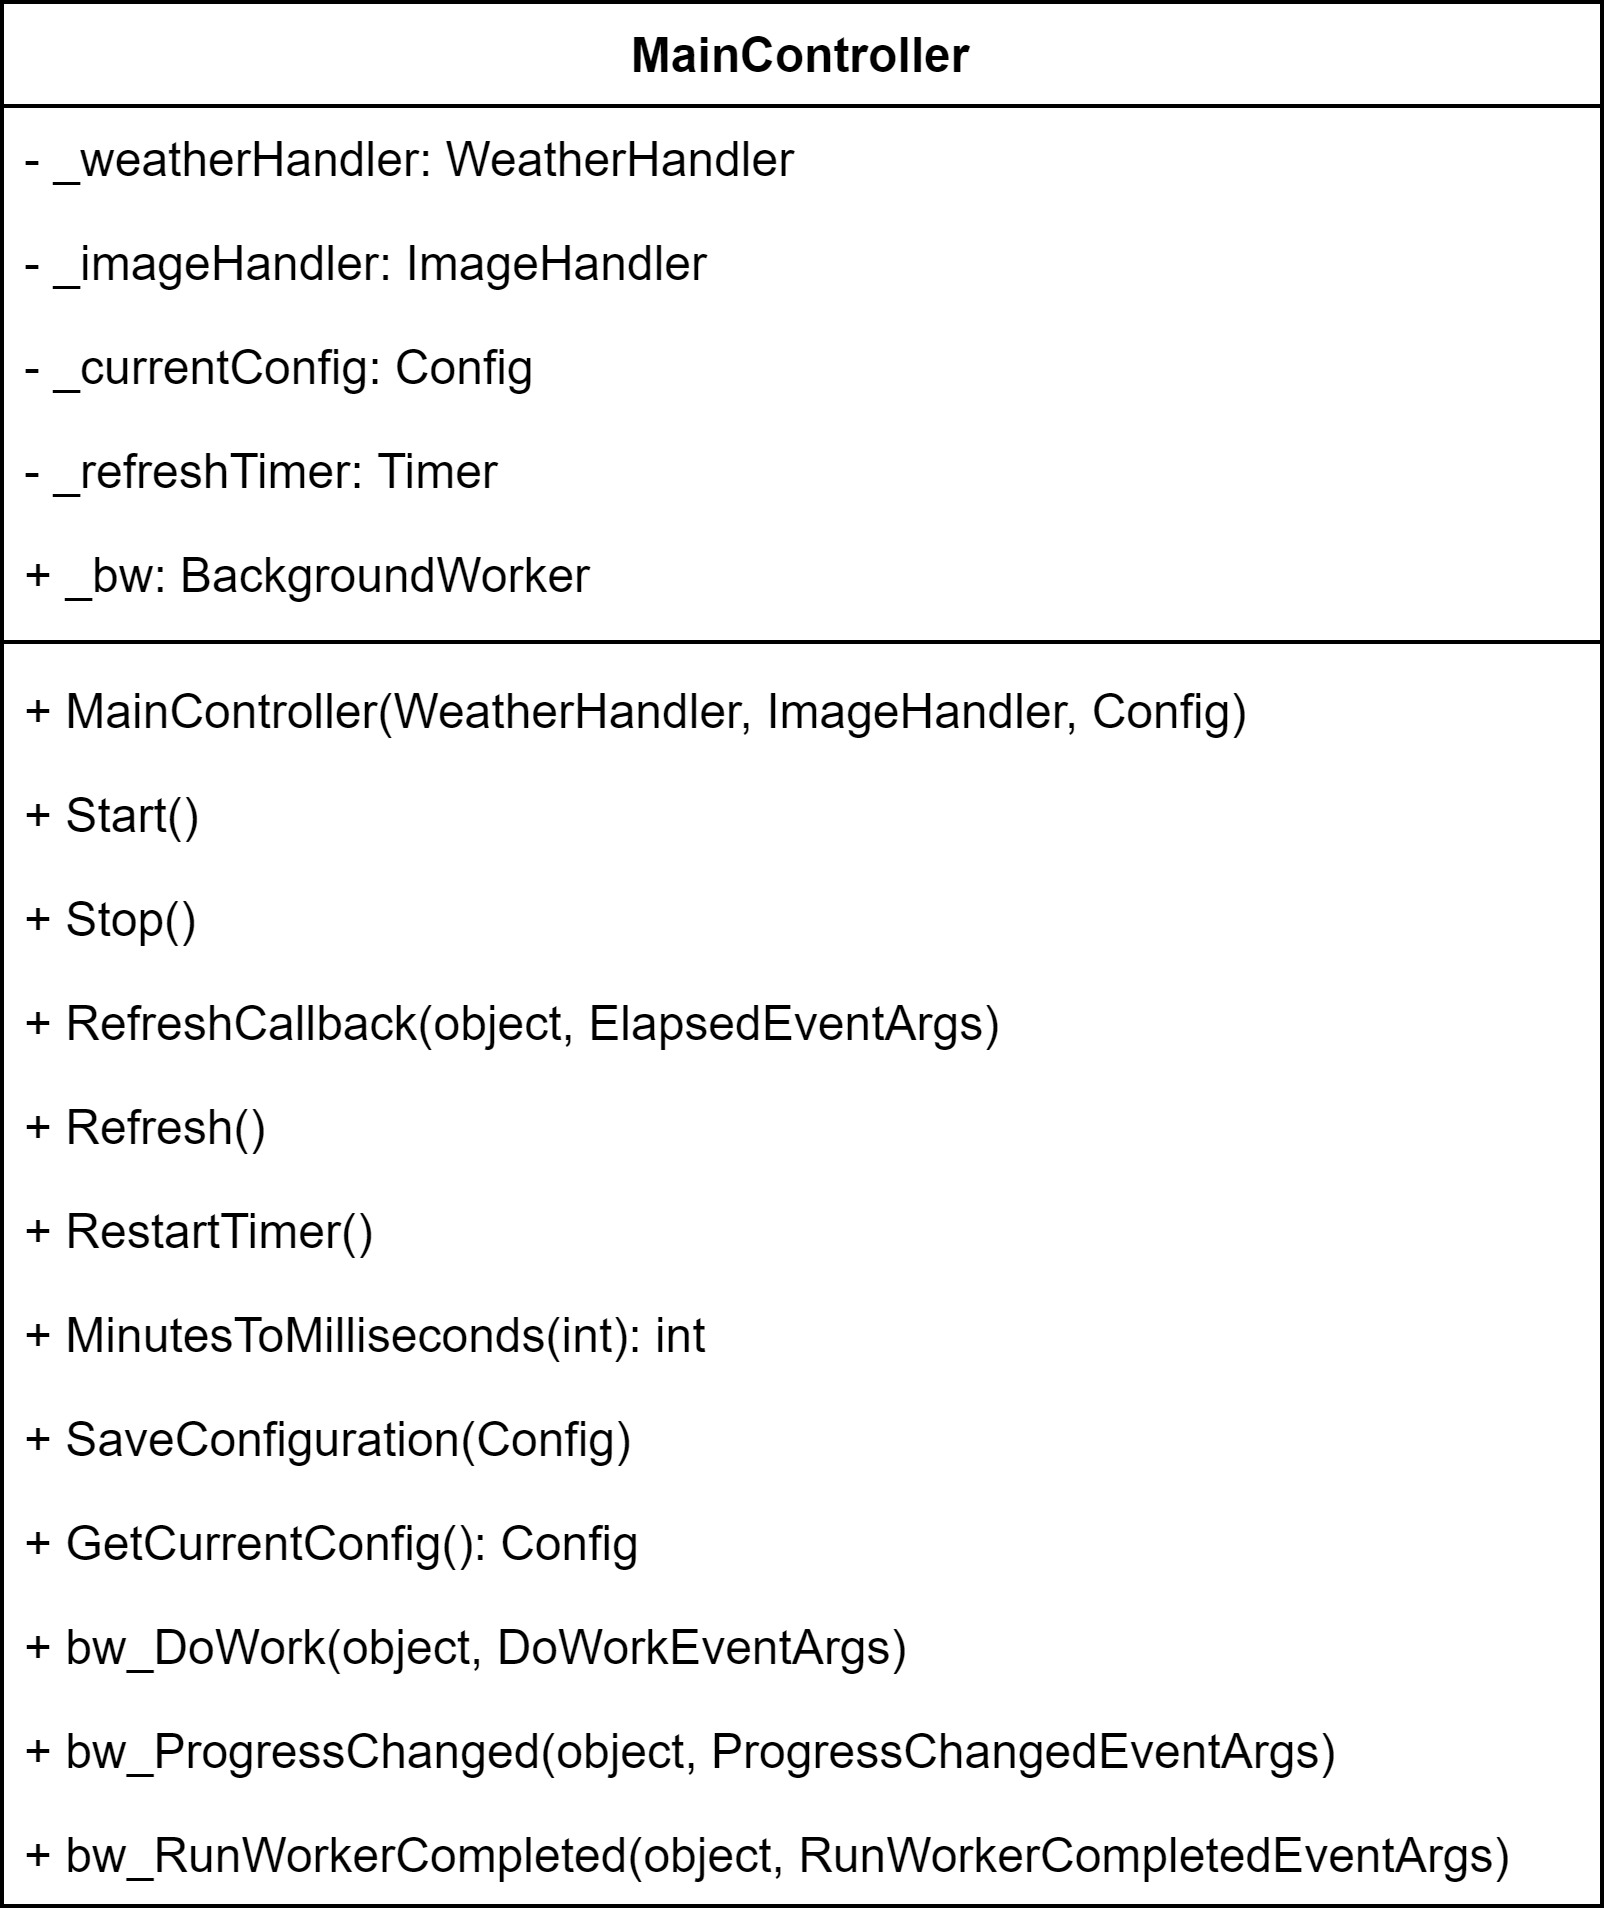
\includegraphics[width=0.5\textwidth]{Bilder/MainController}
\caption[MainController in UML-Form]{\label{MainController} MainController in UML-Form}
\end{figure}

Um diese verschiedenen Responsibilities in neue Klassen aufzuteilen wurden vier neue Klassen entwickelt. Diese werden im Folgenden kurz erläutert. Im \texttt{Refresher} ist die generelle Logik, um den Hintergrund zu aktualisieren ausgelagert. Der \texttt{UpdateTimer} übernimmt das zyklische Aktualisieren des Hintergunds und der \texttt{ScreenChangeWorker} das manuelle Aktualisieren im neuen Thread. In dem neuen \texttt{MainWindowController} wird das Weitergeben der GUI-Inputs an die inneren Schichten umgesetzt. Diese vier Klassen sind \href{https://github.com/Bronzila/WeatherWallpaper/blob/master/CleanArchitecturePics/Architektur_Vorher.jpg}{\color{blue}hier} auf dem UML-Diagramm der Anwendung zu erkennen. Hierbei ist erkennbar, dass der \texttt{MainWindowController}, durch seine Adaptertätigkeiten auch in die Adapter-Schicht bei der Clean Architecture übergegangen ist.

Dann noch ConfigHandler bzw Adapter und Zustand
\subsubsection{Open/Closed Principle}
Das Open/Closed Principle beschreibt, dass Softwäre-Entitäten offen für Erweiterung aber geschlossen bezüglich Veränderung sein sollen. Dementsprechend soll bestehender Code nicht mehr geändert werden. Bei neuen bzw. geänderten Anforderungen wird der bestehende Code also nicht angepasst/geändert, sondern lediglich erweitert.

Bei unserer Anwendung identifiziert man eine mögliche Entwicklung mit Erweiterung klar bei der Validierung der Konfiguration, hier wird also das OCP verletzt. Gerade wenn sich diese in der Zukunft nochmals anpassen sollte, weil bspw. noch weitere Präferenzen des Nutzers/der Nutzerin erfasst werden sollen.
\begin{listing}[h]
\inputminted[linenos=true,frame=lines]{csharp}{Listings/ValidateInputsPre.cs}
\caption{Verletzung des Open/Closed-Principle im ConfigValidator}
\label{ConfigValidatorPre}
\end{listing}
In Listing \ref{ConfigValidatorPre} ist erkennbar, dass der Code zum Überprüfen angepasst werden müsste, falls eine neue Anforderung an die Konfiguration hinzugefügt wird. Daher wird der bisherige \texttt{ConfigValidator} umgeschrieben und hält nun eine \texttt{List<IValidationAspect>}. In dieser Liste sind alle Validierungs-Aspekte gespeichert gegen die die Eingabe getestet werden soll. Das Interface \texttt{IValidationAspect} definiert eine Methode \texttt{Validate(Config)}, welche validiert, ob die Regel eingehalten wurde. Sollte dies nicht der Fall sein, wird eine Exception geworfen. Nun muss im \texttt{ConfigValidator} lediglich über alle registrierten \texttt{IValidationAspects} iteriert werden und mit der übergebenen Config die \texttt{Validate}-Methode aufgerufen werden. Das Hinzufügen einer neuen Anforderung ist nun simpel über das Schreiben einer neuen Klasse möglich. Diese muss \texttt{IValidationAspect} implementieren und auf den \texttt{ConfigHandler} registriert werden. Der neue \texttt{ConfigValidator} und ein Beispiel für einen \texttt{IValidationAspect} ist in Listing \ref{ConfigValidatorPost} zu sehen. Hierbei ist zu beachten, dass bei negativem Testergebnis eine Exception geworfen (und kein false zurückgegeben) wird, um die genaue Fehlerursache dem Nutzer/der Nutzerin mitzuteilen. Wird keine Exception geworfen, ist mit der Konfiguration alles in Ordnung.

\begin{listing}[h]
\inputminted[linenos=true,frame=lines]{csharp}{Listings/ValidateInputsPost.cs}
\caption{Entwicklung mit Erweiterung für den ConfigValidator}
\label{ConfigValidatorPost}
\end{listing}

Ein Punkt an dem das OCP nicht erfüllt ist, ist der \texttt{WeatherInterpreter}. Sollten in Zukunft weitere Daten zur Interpretation des Wetters dazu kommen, so müsste der Code des \texttt{WeatherInterpreters} angepasst und verändert werden.
\subsubsection{Liskov Substitution Principle}
Das Liskov Substitution Principle sagt aus, dass Subtypen sich so wie ihr Basistyp verhalten müssen. Subtypen dürfen daher lediglich die Funktionalität ihres Basistyps erweitern, aber nicht einschränken.
Das Liskov Substitution Principle ist in unserer Anwendung erfüllt, da abgesehen von den verwendeten Interfaces keine Vererbung verwendet wird.
\subsubsection{Interface Segregation Principle}
Das Interface Segregation Principle sagt aus, dass Interfaces passgenau für die aufrufenden Clients sein muss. Das Interface darf also keine Details beinhalten, die der Client gar nicht benötigt.
Die Interfaces unserer Anwendung folgen diesem Prinzip. Anhand des Interfaces \texttt{IFileAccessor} kann man die Entwicklung hin zum Erfüllen des Prinzips gut nachvollziehen, da das Interface \texttt{IFileAccessor} von zwei Klienten verwendet wird. Dabei benötigt einerseits der \texttt{ConfigHandler} den Zugriff auf Dateien (Lesen und Schreiben) und andererseits der \texttt{DownloadHelper} um das Hintergrundbild zu speichern. Das Interface \texttt{IFileAccessor} umfasst daher sowohl das Lesen/Schreiben von Dateien als auch das Schreiben von Bildern. Dieses Interface wurde dementsprechend, um das Interface Segregation Principle zu erfüllen, in zwei Interfaces aufgeteilt. Einerseits das Interface \texttt{IImageWriter} und andererseits das (bereits bestehende) Interface \texttt{IFileAccessor}. Wie der Name schon sagt, kümmert sich das Interface \texttt{IImageWriter} um das Schreiben von Bildern und das Interface \texttt{IFileAccessor} mit dem Lesen und Schreiben von Dateien. In \href{https://github.com/Bronzila/WeatherWallpaper/commit/8db38466c2185e16ef90f71af485e00b57b09032}{\color{blue}diesem Commit} ist das Segmentieren dieser beiden Interfaces zu erkennen.
Generell haben einige Interfaces das ISP nicht erfüllt, allerdings war keins dieser Beispiele so eindringlich wie das Obere, da die meisten Interfaces nur ein aufrufenden Client hatten und auf diesen einzelnen Client nicht passgenau zugeschnitten waren. Mittlerweile wurden auch die Interfaces, die das Prinzip nicht erfüllt haben so umgeschrieben, dass sie es erfüllen.
\subsubsection{Dependency Inversion Principle}
Mit dem Dependency Inversion Principle wird versucht höhere Ebenen von niedrigeren Ebenen zu entkoppeln. Dabei gilt die Regel, dass Abstraktionen nicht von Details abhängen sollen, sondern Details von Abstraktionen abhängen sollten, da Abhängigkeiten auf konkrete Klassen stark koppeln. Sollte dieses Prinzip nicht erfüllt sein, so würden Änderungen in der niedrigeren Ebene Änderungen in der höheren Ebene hervorrufen. Eine Verletzung dieses Prinzips wird mithilfe der Dependency Injection aufgelöst. Dabei sind die Klassen der höheren und niedrigeren Ebene abhängig von einem Interface anstelle von  einer konkreten Klasse. Die Referenz auf die Instanz erhalten die Klassen der höheren Ebene dann meist im Konstruktor.
Die Verletzungen des Dependency Inversion Principle sind bei der Implementierung der Clean Architecture klar auffindbar. Sobald eine innere Schicht eine Abhängigkeit auf eine äußere Schicht hat, wird das Prinzip verletzt. In Kapitel \ref{CleanArchitectureVorher} sind diese Verletzungen nochmals kurz erläutert. Im Folgenden wird beispielhaft die Abhängigkeit vom damaligen \texttt{MainController} (mittlerweile umbenannt in \texttt{Refresher}) auf den \texttt{WeatherHandler}. Hier wird das Prinzip verletzt, da sich der \texttt{Refresher} in der Application Code-Schicht befindet und der \texttt{WeatherHandler} in der Adapter-Schicht. Um dies zu beheben, wird das Interface \texttt{IWeatherHandler} eingesetzt. Der \texttt{WeatherHandler} implementiert dieses und der \texttt{Refresher} hat nur noch die Abhängigkeit auf ein \texttt{IWeatherHandler}. Das tatsächliche Objekt erhält er dann im Konstruktor über Dependency Injection. In Abbildung \ref{DIP} ist dieser kleine Ausschnitt aus dem UML-Diagramm vereinfacht dargestellt und mit Vorher/Nachher betitelt.

\begin{figure}[ht]
\centering
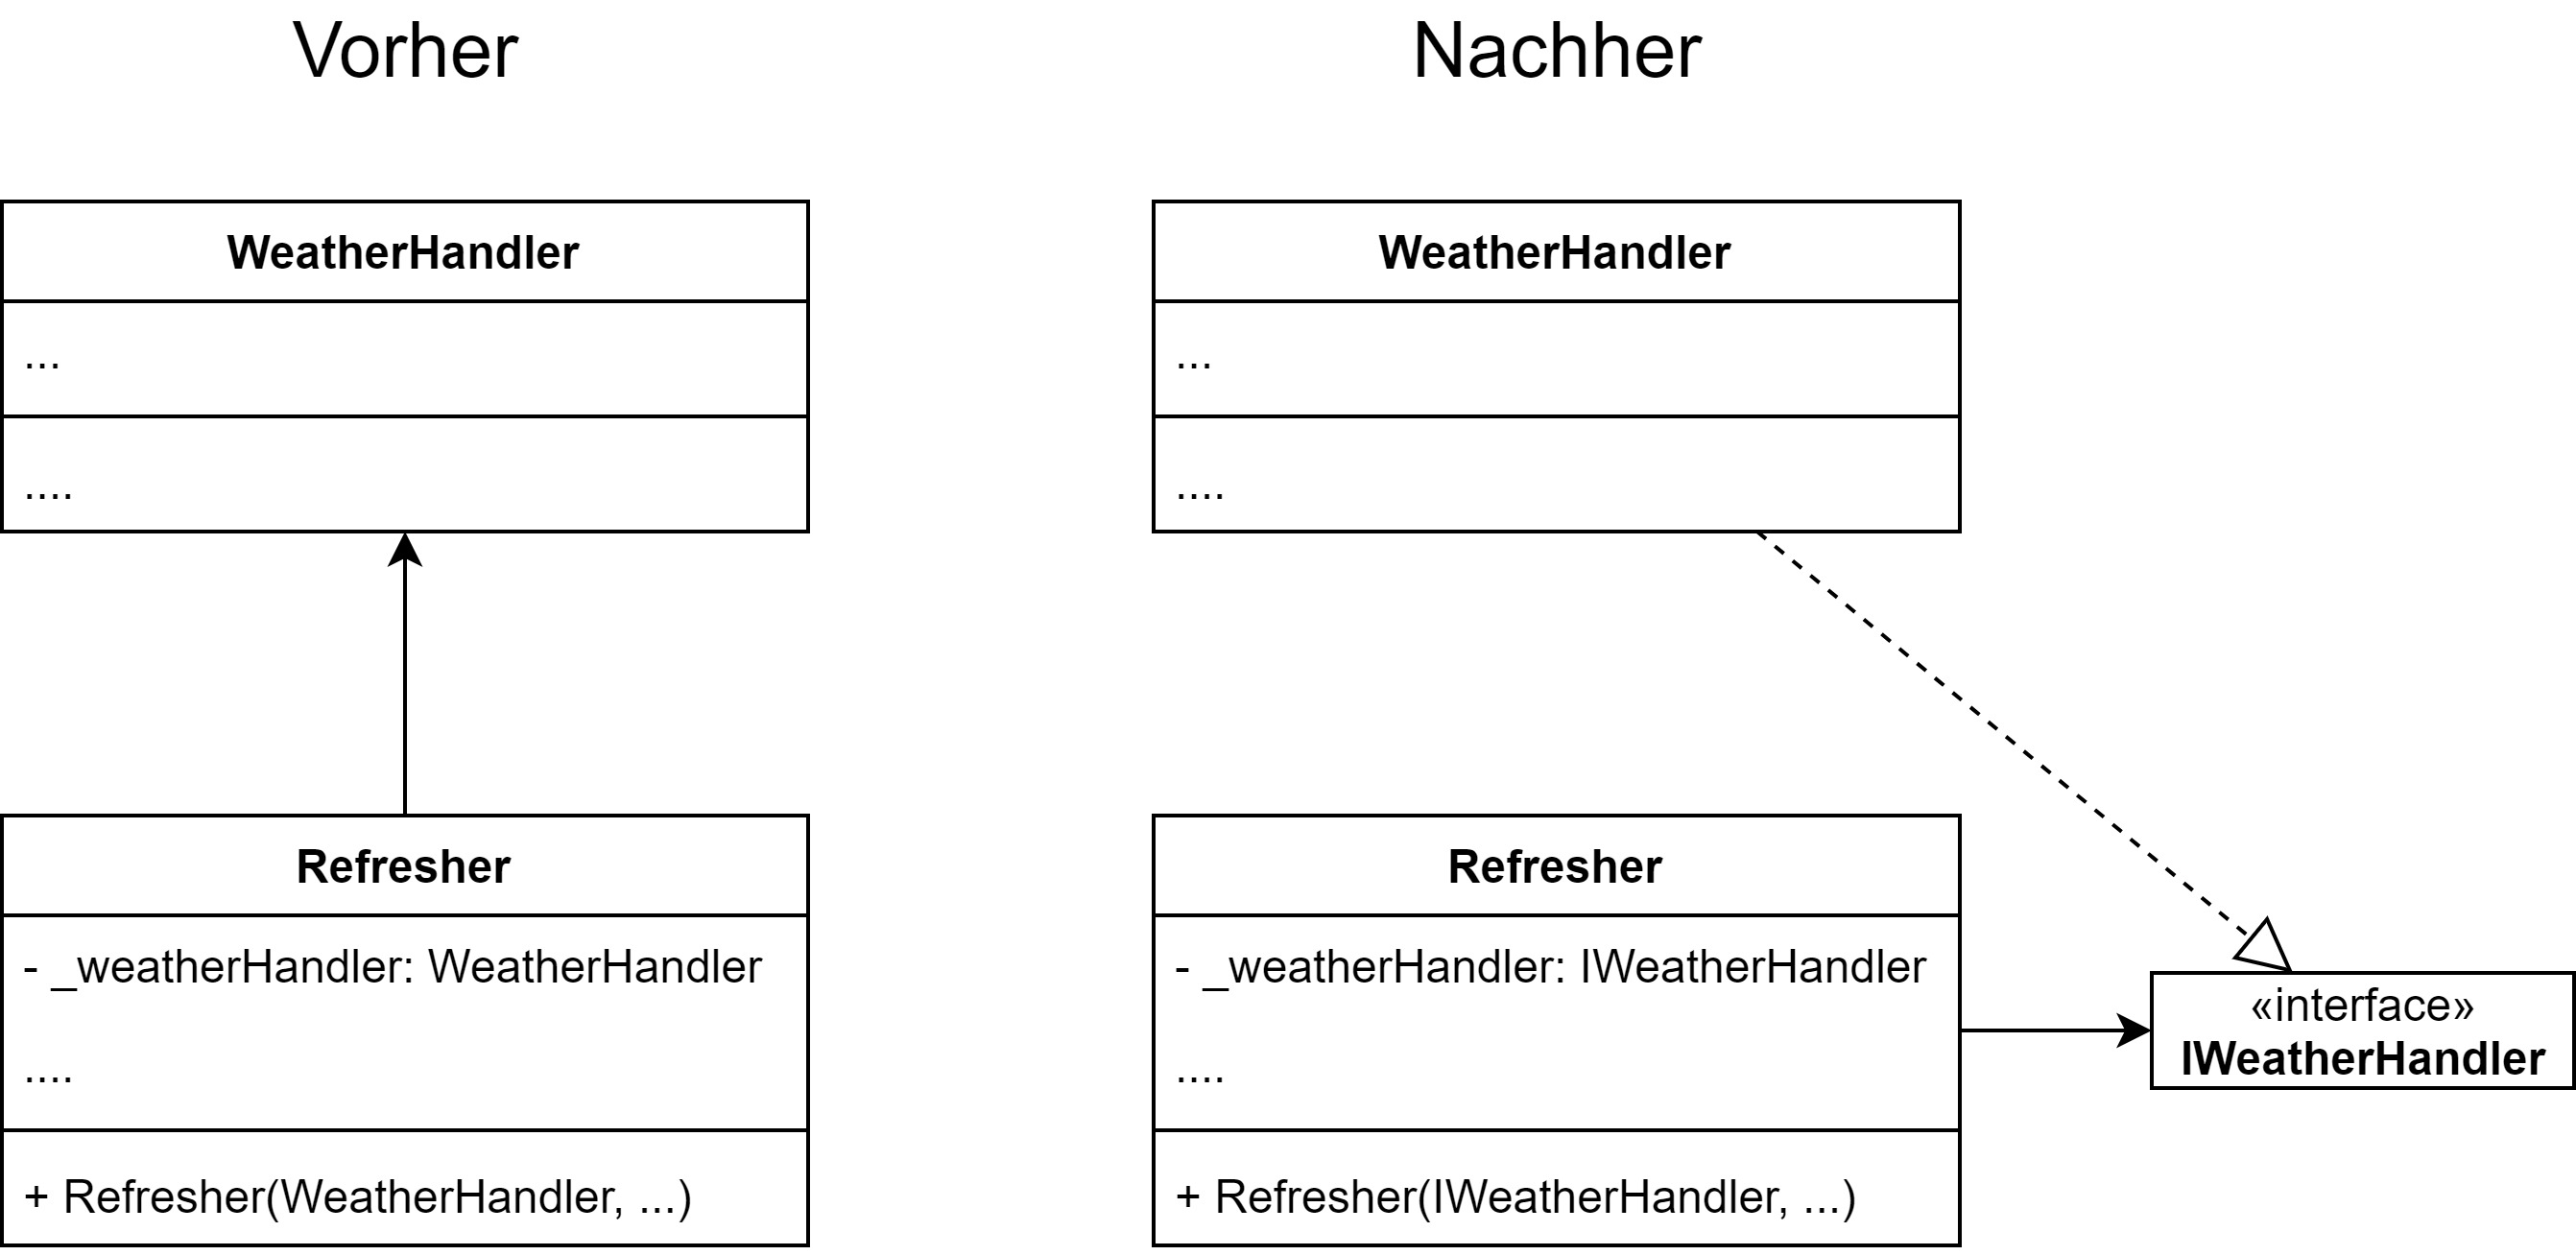
\includegraphics[width=0.8\textwidth]{Bilder/DIP}
\caption[Beispielhafte Verletzung und Verbesserung des DIP]{\label{DIP}Beispielhafte Verletzung und Verbesserung des DIP}
\end{figure}
\subsection{GRASP}

\subsection{DRY}
